%%%%%%%%%%%%%%%%%%%%%%%%%%%%%%%%%%%%%%%%
% University Assignment Title Page
% LaTeX Template
% Version 1.0 (27/12/12)
%
% This template has been downloaded from:
% http://www.LaTeXTemplates.com
%
% Original author:
% WikiBooks (http://en.wikibooks.org/wiki/LaTeX/Title_Creation)
%
% License:
% CC BY-NC-SA 3.0 (http://creativecommons.org/licenses/by-nc-sa/3.0/)
%
% Instructions for using this template:
% This title page is capable of being compiled as is. This is not useful for
% including it in another document. To do this, you have two options:
%
% 1) Copy/paste everything between \begin{document} and \end{document}
% starting at \begin{titlepage} and paste this into another LaTeX file where you
% want your title page.
% OR
% 2) Remove everything outside the \begin{titlepage} and \end{titlepage} and
% move this file to the same directory as the LaTeX file you wish to add it to.
% Then add \input{./title_page_1.tex} to your LaTeX file where you want your
% title page.
%
%%%%%%%%%%%%%%%%%%%%%%%%%%%%%%%%%%%%%%%%%
%\title{Title page with logo}
%----------------------------------------------------------------------------------------
%	PACKAGES AND OTHER DOCUMENT CONFIGURATIONS
%----------------------------------------------------------------------------------------

\documentclass[11pt]{article}
\usepackage[utf8]{inputenc}
\usepackage{amsmath}
\usepackage{graphicx}
%\usepackage{lmodern}
\usepackage{hyperref}
\usepackage{tabularx}
\usepackage{amsmath}
\usepackage{float}
\usepackage[table]{xcolor}
\usepackage{booktabs}% http://ctan.org/pkg/booktabs

\usepackage{fancyhdr}
\usepackage[hscale=0.76,vscale=0.76]{geometry} % Margin sizes
\usepackage{minted} % for this to work: `sudo apt install python-pygments` and use `-shell-escape` flag with `pdflatex`

\newcommand{\tabitem}{~~\llap{\textbullet}~~}
\newcommand{\HRule}{\rule{\linewidth}{0.5mm}} % Defines a new command for the horizontal lines, change thickness here

\pagestyle{fancy}
\fancyhf{}
\rhead{Mission 2 -- Group G}
\lhead{\textit{LINGI2252}}
\cfoot{\thepage}

\begin{document}
    \begin{titlepage}
        \center % Center everything on the page

        %----------------------------------------------------------------------------------------
        %	HEADING SECTIONS
        %----------------------------------------------------------------------------------------

        \textsc{\LARGE Université Catholique de Louvain }\\[0.8cm] % Name of your university/college
        
\includegraphics[scale=0.45]{epl.jpg}
        \\[1.5cm]
        \textsc{\Large LINGI2252}\\[0.5cm] % Major heading such as course name
        \textsc{\large Software Maintenance and Evolution}\\[0.8cm] % Minor heading such as course title

        %----------------------------------------------------------------------------------------
        %	TITLE SECTION
        %----------------------------------------------------------------------------------------

        \HRule \\[0.4cm]
        { \huge \bfseries Mission 2: Improved prototype}\\[0.2cm] % Title of your document
        \HRule \\[1.5cm]

        %----------------------------------------------------------------------------------------
        %	AUTHOR SECTION
        %----------------------------------------------------------------------------------------

		\vfill
        \begin{minipage}{0.4\textwidth}
        \begin{flushleft} \large
        \emph{Authors:}\\
        \textbf{Group G}\\
        \textsc{Gustin}~Simon \\
        1171-14-00\\
        \textsc{Hallet}~Adrien \\
        3276-13-00\\
        \end{flushleft}
        \end{minipage}
        ~
        \begin{minipage}{0.4\textwidth}
        \begin{flushright} \large
        \emph{Professor:} \\
         \textsc{Mens}~Kim \\% Supervisor's Name
         \emph{Assistant:}\\
         \textsc{Duhoux}~Benoît
        \end{flushright}
        \end{minipage}\\[1cm]

        % If you don't want a supervisor, uncomment the two lines below and remove the section above
        %\Large \emph{Author:}\\
        %John~\textsc{Smith}\\[3cm] % Your name

        %----------------------------------------------------------------------------------------
        %	DATE SECTION
        %----------------------------------------------------------------------------------------

        {\large \today}\\[2cm] % Date, change the \today to a set date if you want to be precise

        %----------------------------------------------------------------------------------------
        %	LOGO SECTION
        %----------------------------------------------------------------------------------------

        % Include a department/university logo - this will require the graphicx package

        %----------------------------------------------------------------------------------------

        \vfill % Fill the rest of the page with whitespace
    \end{titlepage}

    \title{AAAAAA}
    \newpage

	\section{Introduction}
		For the course \textit{LINGI2252 -- Software Maintenance and Evolution}, we were asked to improve our first prototype of a house automation system. Specifically, we had to add a parametrization component which would allow us to specify the values and states of the variability points at execution time, a command line interpreter which would allow us to update the state of the house at run time and to use relevant pattern designs to make the code more maintainable. We will discuss each of these extensions.
		
	\section{Parametrization component}
		The first extension we discuss is the parametrization component.
		It allows us to easily change the configuration of a house on two different executions without changing the code.
		It does this in a quite straightforward way: when the program executes, it starts by parsing a configuration file. It then creates a house that corresponds to the configuration described in this file.
		
		As can be expected, the design of this file has the same kind of structure than a house with a given configuration, that is a hierarchical structure. This structure is due to the fact that an automated house can be seen as a group of rooms (in our code \mintinline{java}{HousePart}s), which contain sensors, actuators and connected objects. This hierarchy can actually be seen on our class diagram: a \mintinline{java}{House} is made of \mintinline{java}{HousePart}s which contain \mintinline{java}{Controller}s.
		
		The configuration is contained within an external file formatted in \textit{JSON}. We chose this format for several reasons.
		First, it is well-known and heavily used as a format for configuration files. It is thus totally capable of handling this kind of task. If we had decided to make our own "configuration language", we could have very easily ended up with a syntax that would not fit all possible configurations perfectly, or with a flawed parser that would not work in certain cases.

		Secondly, the fact that it is a well-known format also means that parsers exist in most languages. We didn't have to implement one by ourselves or to use an incomplete or buggy implementation.

		Lastly, we are used to this format, which means we can work quickly and efficiently with it. The likelihood of us making an error while using it was thus smaller. This being said, using \textit{YAML} or \textit{TOML} would be perfectly legitimate choices, but we weren't as used to them as we are to \textit{JSON}. Note that using the latter instead of one of those two formats prevents us from having comments in our configuration files, which can be considered a problem.
		
		Notice that we didn't decide to implement the parser as a class of its own but rather to place the parsing logic inside the class \mintinline{java}{House}. As we use an external library to parse the configuration file, we figured out it wouldn't be very interesting to make a parser that would be only a couple of lines long. The configuration of the house is then done from within this class itself on basis of the parsed representation of the file. However, if we needed to parse files in other formats, making a class to handle the parsing would be a very good idea.
	
	\section{Command line interpreter}
		We discuss now the second extension we implemented, i.e. the command line interpreter. As we already said, this extension can be used to update the state of the house by typing commands during the execution of the program.
		
		Each command is quite simple to interpret with the first word corresponding to the action to execute and the following words being the (optional) parameter(s) of the action. We designed them this way in order to simplify the implementation of the interpreter: it simply test whether it recognizes the first word and calls a subsequent method accordingly, giving it the remaining words as arguments. This implementation is made in a class named \mintinline{java}{Scenario}. 
		
		A specificity of our implementation is also that commands can be received in two different ways: either sequentially from the standard input, or from an input file which contains one command per line. The behavior is then similar in both cases, the program interpreting and executing one command at a time in the order they are given.
		
		To make the code more reusable, we separated the interpretation of commands and the actions performed afterwards. Indeed, when a command is interpreted, the code calls a method that represents the action associated with this particular command. This improves reusability since it allows us to change the interpreter logic (for example, to create a different interpreter that would support another language or to add commands that would map to the same actions) and still be execute the exact same code for similar cases. It also makes our code easier to improve as adding a new command would be very easy. Finally, making it this way makes our code more readable.

  \section{Variability Points}
    \subsection{House Layout}
      The main variability point is the ability to adapt each possible house. Our application can modify the house layout via the parametrization component. Thanks to the \texttt{HousePart} component, we can split the \texttt{House} in as many subcomponents as we want (either one per floor, one per room, one per square meter, whatever fits the needs). The implementation is pretty straightforward as the \texttt{House} is nothing but a dynamic list of \texttt{HousePart}.
      \begin{minted}[autogobble]{java}
        public class House{
          private static House instance;
          private static String filename;

          JSONObject config;
          ArrayList<HousePart> housePartList;
          ...
        }
      \end{minted}

    \subsection{Controllers}
      In the configuration file, you can also modify the controllers (sensors, actuators and connected objects). You can place them and link a sensor to one or multiple actuators and/or connected objects. With such an implementation, you can link any kind of supported event (\emph{e.g.: detecting motion, smoke, humidity, ...}) to any kind of supported action (\emph{e.g.: opening a door, turning a light on, ...}). As for the house layout, this has been done with a simple dynamic list of \texttt{Sensor} linking to a dynamic list of \texttt{Actuator} in a \texttt{HousePart}.
      \begin{minted}[autogobble]{java}
        HousePart(House parent, JSONObject housePart){
          ...
          if (housePart.has("actuators"))
              this.actuators = parseActuators(housePart.getJSONArray("actuators"));
          else
              this.actuators = new Actuator[0];
          if (housePart.has("objects"))
              this.connectedObjects = parseConnectedObjects(housePart.getJSONArray("objects"));
          else
              this.connectedObjects = new ConnectedObject[0];
          if (housePart.has("sensors"))
              this.sensorsJSON = housePart.getJSONArray("sensors");
          else
              this.sensors = new Sensor[0];
          ...
      \end{minted}

    \subsection{Disable controllers}
      This one is self-explanatory. You can dynamically disable/enable controllers at runtime, effectively changing the observable behavior of the system. This is simply a clever use of boolean conditions modified by the running \texttt{Scenario} within the \texttt{HomeController}.
      \begin{minted}[autogobble]{java}
      public abstract class Controller {
        public String type;
        public double value = 0.0;
        private boolean enabled = true;
        private boolean inverted = false;
        ...
      }
      \end{minted}

    \subsection{Inverting controllers}
      Maybe you don't want an action to execute when a sensor is triggered, but when it is not. In the parametrization component, you can define an inverted sensor. This effectively doubles the possibilities as each sensor can now have two different behaviors. For example, you could want your door to close when the humidity sensor detects rain. Once again, the implementation is simple with a boolean condition checking if the \texttt{Sensor} is inverted.
      \begin{minted}[autogobble]{java}
      static void triggerActions(Sensor sensor){
          Actuator[] aList = sensor.getActuatorList();
          for(Actuator cActuator : aList){
              ...
              else { // Trigger one in given housePart
                  if (!sensor.isInverted())
                      cActuator.trigger();
                  else
                      cActuator.reset();
              }
          }
      }
      \end{minted}

  \section{Design Patterns}
    \subsection{Abstract Factory}
      We have three factories to create the controllers. \texttt{SensorFactory}, \texttt{ActuatorFactory}, \texttt{ConnectedObjectFactory}. We do not have a higher-level factory because it would only reduce readability in the context.
      \begin{figure}[!h]
        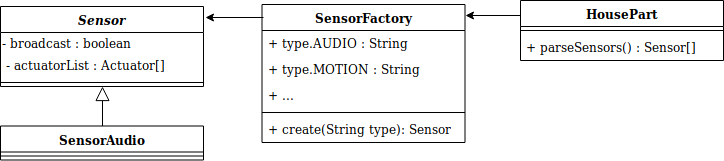
\includegraphics[width=\textwidth]{sensorfactory.png}
      \end{figure}

	\section{Conclusion}

\end{document}
